\section{Zielsetzung}
Das Ziel dieses Versuches ist die Bestimmung der Zeitkonstante eines RC-Kreises, sowie die Messung der Amplitude der Kondensatorspannung
und der Phasenverschiebung zwischen Generator- und Kondensatorspannung, jeweils in Abhängigkeit der Generatorfrequenz. Der letzte Teil des
Versuches befasst sich mit der Eigenschaft des RC-Kreises als Integrator.
%---------------------------------------------------------------
\section{Theorie}

\subsection{Allgemeine Relaxationsgleichung und Anwendung auf den RC-Kreis}
Als Relaxationserscheinung wird das nicht-oszillatorische Zurückkehren eines Systems in seinen Grundzustand bezeichnet, nachdem das System 
angeregt wurde. Wird eine Größe A beobachtet, so ist die Änderungsgeschwindigkeit proportional zur Abweichung von A zum 
Endzustand $\text{A}(\infty)$:

\begin{equation*}
\frac{\symup{d}A}{\symup{dt}} = c[A(t) -A(\infty)].
\end{equation*}
Wird über die Zeit 0 bis t integriert, so ergibt sich

\begin{equation}
\begin{aligned}
&\int_{A(0)}^{A(t)} \frac{\symup{d}A'}{A' - A(\infty)} = \int_0^t c \, \symup{d}t' \\
&\iff \symup{ln} \frac{A(t) - A(\infty)}{A(0) - A(\infty)} = ct \\
\end{aligned}
\end{equation}

\begin{equation}
\iff A(t) = A(\infty) + [A(0) - A(\infty)] \cdot e^{ct}.
\label{eq:groesseA}
\end{equation}
In einem RC-Kreis sind Relaxationserscheinungen bei der Auf- und Entladung des Kondensators über den Widerstand zu beobachten.
\begin{figure}[h!]
	\centering
	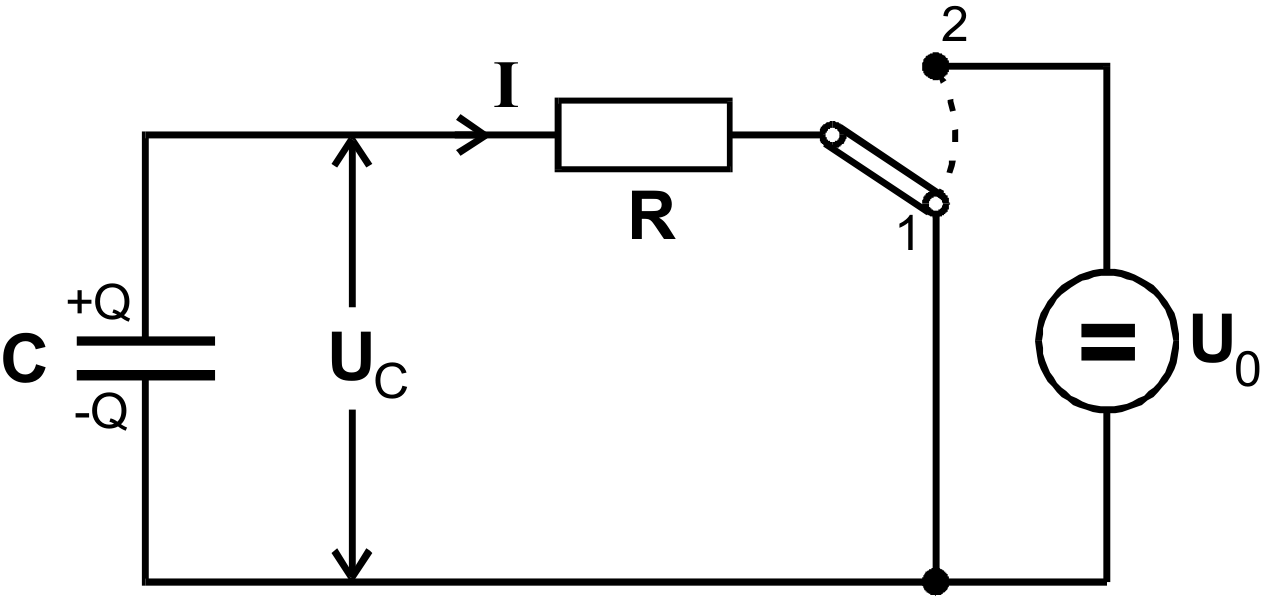
\includegraphics[scale=.3]{content/RC-Kreis}
	\caption{Entladung (1) und Aufladung (2) des Kondensators über den Widerstand, \cite[1]{anleitung353}.}
	\label{fig:rc-kreis}
\end{figure}
\subsubsection{Entladevorgang}
\label{eq:entladung}
Sei $Q$ die Ladung auf den Platten eines Kondensators mit der Kapazität $C$, so lässt sich die Spannung $U_{\text{C}}$ mit
\begin{equation}
U_{\text{C}} = \frac{Q}{C}
\label{eq:spannungc}
\end{equation}
bestimmen. Weiter ist nach dem Ohmschen Gesetz der Strom $I$ durch den Widerstand $R$ gegeben mit
\begin{equation}
I = \frac{U_{\text{C}}}{R}.
\label{eq:strom}
\end{equation}
Beim Ladungsausgleich fließt die Ladung $I \symup{d}t$ von einer Kondensatorplatte zur anderen über, was eine Ladungsänderung auf den Platten von 
\begin{equation}
\symup{d}Q = -I\,\symup{d}t
\label{eq:ladungsanderung}
\end{equation}
herbeiführt. Mit \eqref{eq:spannungc}, \eqref{eq:strom} und \eqref{eq:ladungsanderung} lässt sich nun eine Differentialgleichung aufstellen, 
die den zeitlichen Verlauf der Ladung des Kondensators beschreibt:
\begin{equation*}
\frac{\symup{d}Q}{\symup{d}t} = -\frac{1}{RC}\cdot Q(t).
\end{equation*}
Nach unendlich langer Zeit hat sich der Kondensator vollständig entladen, also gilt
\begin{equation*}
Q(\infty) = 0,
\end{equation*}
sodass sich nach Integration, analog zu \eqref{eq:groesseA}
\begin{equation}
\label{eqn:Meth1}
Q(t) = Q(0)\cdot e^{-\frac{t}{RC}}
\end{equation}
ergibt.

\subsubsection{Aufladevorgang}
Analog zu \eqref{eq:entladung} kann die Gleichung für den Aufladevorgang mit den Randbedingungen 
\begin{equation*}
\begin{aligned}
Q(0) &= 0 \\
Q(\infty) &= C\cdot U_{\text{C}} \\
\end{aligned}
\end{equation*}
zu 
\begin{equation*}
Q(t) = C\cdot U_{\text{C}} (1- e^{-\frac{t}{RC}})
\end{equation*}
berechnet werden.

In den Gleichungen für den Auf- und Entladevorgang ist $RC$ eine Zeitkonstante, die angibt, wie lange ein System braucht, 
um auf $\frac{1}{e} \approx 36{,}8\%$ seines Ausgangswertes zu kommen.

%---------------------------------------------------------------


\subsection{Relaxationserscheinungen bei periodischer Auslenkung aus der Gleichgewichtslage}

In einem RC-Kreis erfolgt eine periodische Anregung durch eine äußere Wechselspannung $U(t)$ mit
\begin{equation*}
U(t) = U_{\text{C}}\cdot \symup{cos}(\omega t).
\end{equation*}
Hierbei gilt, dass U(t) gleich $U_{\text{C}}$ ist wenn die Kreisfrequenz $\omega$ gering ist, also wenn gilt: $\omega \ll \frac{1}{RC}$.

Desweiteren gilt, dass mit höheren Kreisfrequenzen die Auf- und Entladung des Kondensators aufgrund des Widerstandes zunehmend hinter der 
angelegten Generatorspannung zurückliegen. Daraus ergibt sich eine Phasenverschiebung 
$\varphi$ zwischen den beiden Spannungen und eine abnehmende Amplitude $A$ der Spannungskurve des Kondensators.

Die Frequenzabhängigkeit von Phasenverschiebung und Amplitude kann mit dem Ansatz
\begin{equation*}
U_{\text{C}} = A(\omega)\cdot \symup{cos}(\omega t + \varphi \{\omega\})
\end{equation*}
ermittelt werden. 

Mit dem 2. Kirchhoffschen Gesetz
\begin{equation*}
\begin{aligned}
U(t) &= U_{\text{R}} + U_{\text{C}} \\
\implies U_0 \cdot \symup{cos}(\omega t) &= I(t)\cdot R + A(\omega)\cdot \symup{cos}(\omega t + \varphi).
\end{aligned}
\end{equation*}
und 
\begin{equation}
I(t) = \frac{\symup{d}Q}{\symup{d}t} = C \frac{\symup{d}U_{\text{C}}}{\symup{d}t}
\label{eq:strom2}
\end{equation}
folgt:
\begin{equation}
U_{\text{C}}\cdot \symup{cos}(\omega t) = -A\omega RC\cdot \symup{sin}(\omega t + \varphi) + A(\omega)\cdot \symup{cos}(\omega t + \varphi).
\label{eq:langegleichung}
\end{equation}
Wird nun in \eqref{eq:langegleichung} $\omega t = \frac{\pi}{2}$ gesetzt, sowie 
$\symup{sin}(\varphi + \frac{\pi}{2}) = \symup{cos}(\varphi)$ und $\symup{cos}(\varphi + \frac{\pi}{2}) = -\symup{sin}(\varphi)$,
so ergibt sich die Phasenverschiebung in Abhängigkeit der Frequenz mit

\begin{equation}
\varphi(\omega) = \symup{arctan}(-\omega RC).
\label{eq:phasenverschiebung}
\end{equation}
Zu sehen ist, dass die Phasenverschiebung für niedrigere Frequenzen abnimmt und für hohe Frequenzen gegen $\frac{\pi}{2}$ strebt.

Für $\omega t + \varphi = \frac{\pi}{2}$ folgt aus \eqref{eq:langegleichung}:
\begin{equation}
A(\omega) = -\frac{\symup{sin}\varphi}{\omega RC}\cdot U_0.
\label{eq:amplitudezwischen}
\end{equation}
Aus \eqref{eq:phasenverschiebung} und $\symup{sin}^2 \varphi + \symup{cos}^2 \varphi = 1$ ergibt sich

\begin{equation*}
\symup{sin}\varphi = \frac{\omega RC}{\sqrt{1+\omega^2 R^2 C^2}}.
\end{equation*}
Wird dies in \eqref{eq:amplitudezwischen} eingesetzt, so ist das Ergebnis die Gleichung für die Amplitude in Abhängigkeit der Frequenz:
\begin{equation}
\label{eq:Meth2}
A(\omega) = \frac{U_0}{\sqrt{1+\omega^2 R^2 C^2}}.
\end{equation}
Es ist zu erkennen, dass die Amplitude für kleine Kreisfrequenzen gegen $U_0$ geht und für hohe Frequenzen verschwindet.

%---------------------------------------------------------------

\subsection{Der RC-Kreis als Integrator}

Unter bestimmten Bedingungen kann eine Spannung $U(t)$ mit dem RC-Kreis integriert werden. Wird dazu in das 2. Kirchhoffsche Gesetz
\begin{equation*}
U(t) = U_{\text{R}}(t) + U_{\text{C}}(t) = I(t)\cdot R + U_{\text{C}}(t)
\end{equation*}
die Gleichung \eqref{eq:strom2} eingesetzt, so folgt:
\begin{equation*}
U(t) = RC\cdot \frac{\symup{d}U_{\text{C}}(t)}{\symup{d}t} + U_{\text{C}}(t) \\
\end{equation*}

Mit $\omega \gg \frac{1}{RC}$ ist $|U_{\text{C}}| \ll |U_{\text{R}}|$ und $|U_{\text{C}}| \ll |U|$ und es ergibt sich die Näherung
\begin{equation*}
\begin{aligned}
U(t) &= RC\cdot \frac{\symup{d}U_{\text{C}}(t)}{\symup{d}t} \\
\iff U_{\text{C}}(t) &= \frac{1}{RC} \int_0^t U(t')\, \symup{d}t'.
\end{aligned}
\end{equation*}
